\documentclass[tikz, border=2pt]{standalone}

\usepackage{amsmath,amssymb}
\usepackage{pgfplots}
\pgfplotsset{compat=1.18}
\usepgfplotslibrary{groupplots}
\usepackage{xcolor}

\definecolor{utnblue}{RGB}{0, 51, 102}
\definecolor{utnred}{RGB}{204, 0, 0}

\begin{document}
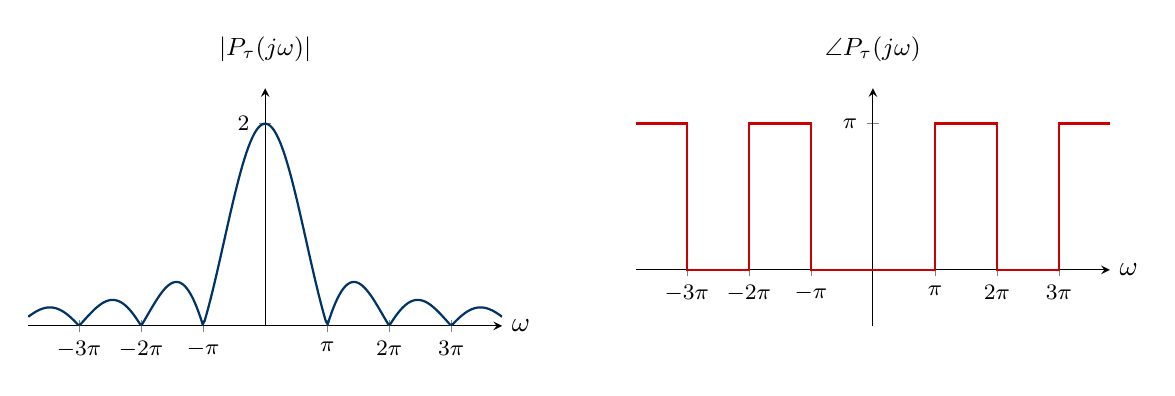
\begin{tikzpicture}

\begin{groupplot}[
    group style={group size=2 by 1, horizontal sep=1.7cm},
    width=7.6cm, height=4.6cm,
    axis lines=middle,
    enlargelimits=false,
    tick label style={font=\footnotesize},
    label style={font=\small},
    title style={font=\small},
    every axis x label/.style={at={(ticklabel* cs:1)}, anchor=west},
]

% --- Panel 1: modulo |P| ---
\nextgroupplot[
    title={$|P_\tau(j\omega)|$},
    xlabel={$\omega$},
    xmin=-12, xmax=12, ymin=0, ymax=2.35,
    xtick={-9.4248,-6.2832,-3.1416,3.1416,6.2832,9.4248},
    xticklabels={$-3\pi$,$-2\pi$,$-\pi$,$\pi$,$2\pi$,$3\pi$},
    ytick={2}, yticklabels={$2$},
]
\addplot[utnblue, thick, samples=240, domain=-12:12] {abs(2*sin(deg(x))/x)};

% --- Panel 2: fase angP ---
\nextgroupplot[
    title={$\angle P_\tau(j\omega)$},
    xlabel={$\omega$},
    xmin=-12, xmax=12, ymin=-1.2, ymax=3.9,
    xtick={-9.4248,-6.2832,-3.1416,3.1416,6.2832,9.4248},
    xticklabels={$-3\pi$,$-2\pi$,$-\pi$,$\pi$,$2\pi$,$3\pi$},
    ytick={0,3.1416}, yticklabels={$0$,$\pi$},
]
\addplot[utnred, thick] coordinates {
  (-12,3.1416) (-9.4248,3.1416) (-9.4248,0) (-6.2832,0)
  (-6.2832,3.1416) (-3.1416,3.1416) (-3.1416,0) (3.1416,0)
  (3.1416,3.1416) (6.2832,3.1416) (6.2832,0) (9.4248,0)
  (9.4248,3.1416) (12,3.1416)
};

\end{groupplot}

\end{tikzpicture}
\end{document}
